\section{Trace Lifetime Analysis}
To be able to predict the remaining time until a failure, it is helpful to know how the lifetime of the traces is distributed. In this section we will attempt to fit the lifetime of the traces to a distribution.

\subsection{Normality}
The first guess for a fitting distribution would be a normal distribution. However, the Shapiro-Wilk normality test rejected the hypothesis that the lifetimes are normally distributed with a p-value of $1.26\times 10^{-5}$. Hence, we can safely conclude that the data do not follow a normal distribution. This is also visible on the following quantile-quantile plot.
\begin{figure}[H]
\centering
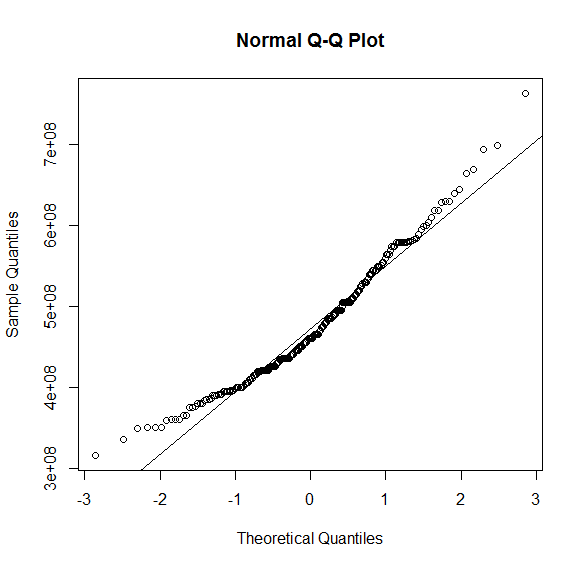
\includegraphics[width=0.8\textwidth]{Plots/QQPlot.png}
\caption{Quantile-quantile plot of the trace lifetimes.}
\end{figure}

\subsection{Cullen and Frey graph}
\begin{figure}[H]
\centering
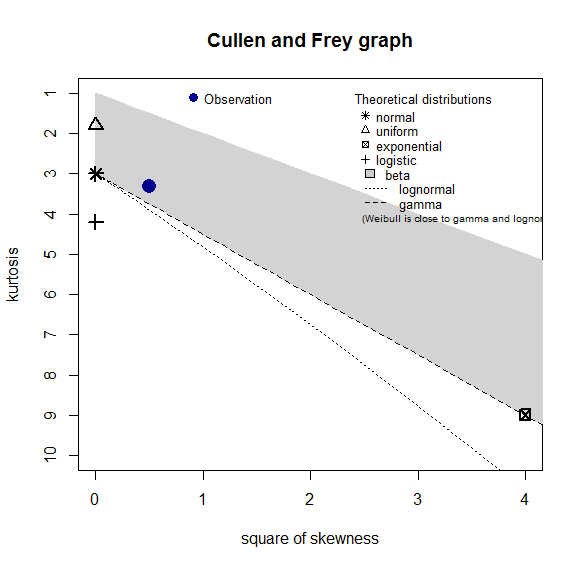
\includegraphics[width=0.8\textwidth]{Plots/CullenAndFray.png}
\caption{Cullen and Fray graph of the data.}
\end{figure}
Above, a Cullen and Fray graph is plotted. The data is placed based on its kurtosis and skewness. A few well-known distributions are also plotted on this plane. This plot would suggest a beta distribution. However, the beta distribution has a support of $[0,1]$ while the lifetime of a trace is not bounded. Other distributions that have similar kurtosis and skewness are the Weibull distribution and the gamma distribution.\\
After estimating the parameters for each of these distributions and performing a Anderson-Darling Goodness-of-Fit test, the gamma-distribution seems to fit the data best with a p-value of $0.195$ versus a $p$-value of $0.00444$. Below, the cumulative gamma distribution with these parameters is plotted over the observed data.
\begin{figure}[H]
\centering
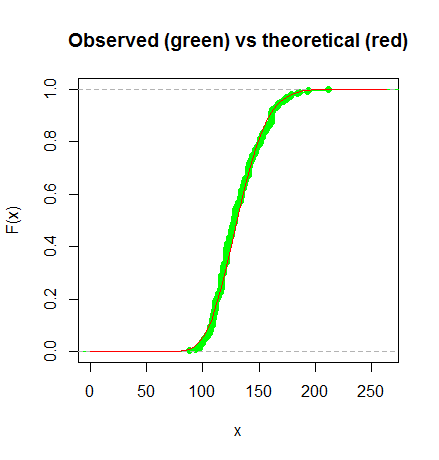
\includegraphics[width=0.8\textwidth]{Plots/GammaCDF.png}
\caption{The gamma distribution plotted over the data.}
\end{figure}